\hfill \bigbreak
Svaki noviji usmjeritelj ima ugrađen firewall kojem je uloga spriječiti internetskom prometu ulazak u lokalnu mrežu usmjeritelja. Zbog takvog ponašanja nije moguć udaljeni pristup uređajima unutar te mreže pa je potrebno na neki način dati do znanja usmjeritelju da ipak propusti naše podatke do ciljanog uređaja. Način na koji se to radi zove se prosljeđivanje porta, poznatije kao port forwarding, što je posebna konfiguracija nadležnog usmjeritelja.

Kada bismo podatke poslali na ciljani uređaj (npr. Uređaj1 na slici \ref{fig:port}) s udaljene adrese naš usmjeritelj ne bi znao na koju IP adresu proslijediti podatke. Zbog toga je potrebno konfigurirati usmjeritelj tako da mu zadamo točne IP adrese i portove na koje će proslijediti podatke koji stignu s interneta. 
\begin{figure}[h!]
	\centering
     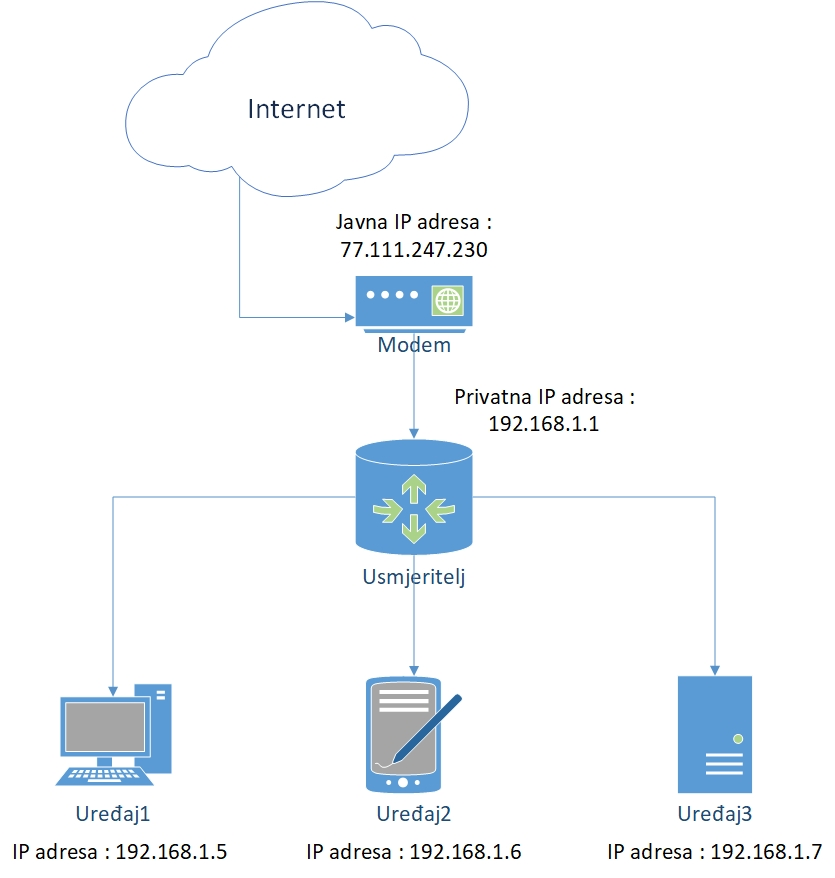
\includegraphics[width=0.8\textwidth]{port}
     \caption{Primjer lokalne mreže}
     \label{fig:port}
\end{figure}
\FloatBarrier
\smallbreak
U daljnjim poglavljima prilikom uspostave veze između klijenta i VPN servera važna je mogućnost povezivanja udaljenog korisnika i VPN servera. U svakom od slučajeva korisnik se nalazi negdje u internetu i želi se povezati na server koji ima lokalnu IP adresu na primjer 192.168.1.5. Ono što je potrebno znati prilikom postavljanja prosljeđivanja porta je IP adresa servera (u ovom slučaju 192.168.1.5), port na kojem server sluša i port s kojeg podaci dolaze.

Prosljeđivanje se započinje tako da se ode u postavke usmjeritelja. Najčešće se to radi tako da se u web preglednik upiše adresa nadležnog usmjeritelja 192.168.1.1 kao na slici. U postavkama je potrebno pronaći prosljeđivanje podataka te dodati novu mogućnost prosljeđivanja kako bi se omogućilo povezivanje na ciljani uređaj. Važno je naglasiti da je potrebno imati pristup usmjeritelju te da svaki usmjeritelj ima svoj način kako se postavljaju navedena svojstva. Detaljnije se upute mogu pronaći na službenim stranicama proizvođača usmjeritelja.
